\documentclass[11pt,aspectratio=43,t]{beamer}

% -------------------------------------------------
% Theme and appearance
% -------------------------------------------------

\usetheme{Madrid}
\usecolortheme{default}
\setbeamertemplate{blocks}[rounded]
% Keep slides clean
\setbeamertemplate{navigation symbols}{}
\setbeamertemplate{footline}{}

% Wider margins for readability
\setbeamersize{text margin left=1.4cm, text margin right=1.4cm}

% Title hierarchy
\setbeamerfont{title}{series=\bfseries}
\setbeamerfont{frametitle}{series=\bfseries,size=\large}

% Bullet style and spacing (discourages overfull slides)
\setbeamertemplate{itemize items}[circle]
\setlength{\itemsep}{0.7em}
\setlength{\parskip}{0.3em}

% Do nothing automatically at new sections (we use explicit divider frames)
\AtBeginSection{}

% -------------------------------------------------
% Maths and graphics
% -------------------------------------------------
\usepackage{amsmath,amssymb}
\usepackage{graphicx}
\graphicspath{
  {figures/}
%  {figures/chap1/}
}
\usepackage{makecell}
\usepackage{booktabs}
% Optional: set your default figure path(s) here if you like
% \graphicspath{{figures/}{figures/lectures/}}



% -------------------------------------------------
% Title information (override per lecture file)
% -------------------------------------------------
\title[Geometry Without Manifolds]{What Becomes of Geometry\\When the Manifold Is Gone?}
%\subtitle{Combinatorial Mesh Calculus}
\author{\href{https://scholar.google.co.uk/citations?user=3nWJe5wAAAAJ&hl=en}{\textbf{Andrey Jivkov}}}
\institute{Department of Mechanical and Aerospace Engineering\\
The University of Manchester}
\date{\today}


% -------------------------------------------------
% Custom slide types / helpers
% -------------------------------------------------

% Title slide helper (so lecture files stay short and consistent)
\newcommand{\maketitleslide}{
\begin{frame}
  \titlepage
\end{frame}
}

% Overview slide helper (accepts an itemize body)
\newcommand{\overviewframe}[1]{
\begin{frame}{What this lecture is about}
\begin{itemize}
  #1
\end{itemize}
\end{frame}
}

% Section divider slide
\newcommand{\sectionframe}[1]{
\begin{frame}[plain]
  \vfill
  \centering
  {\Large\bfseries #1}
  \par\vspace{0.5em}
  \rule{0.4\textwidth}{0.4pt}
  \vfill
\end{frame}
}

% Figure placeholder slide
\newcommand{\figureframe}[1]{
\begin{frame}{}
  \centering
  \vspace{1.0cm}
  \textit{[Figure placeholder: #1]}
\end{frame}
}

% Figure + text frame (left text, right figure placeholder)
% #1 = frame title
% #2 = left content (typically itemize, keyidea, short text)
% #3 = figure description
\newcommand{\figtextframe}[3]{
\begin{frame}{#1}
\begin{columns}[T]
  \begin{column}{0.52\textwidth}
    #2
  \end{column}
  \begin{column}{0.46\textwidth}
    \centering
    \vspace{0.2em}
    \textit{[Figure: #3]}
  \end{column}
\end{columns}
\end{frame}
}

% Key idea emphasis (keep it short; do not paste full definitions)
\newenvironment{keyidea}{
\begin{itemize}
  \item[\textbf{Key idea}]
}{
\end{itemize}
}

% Summary slide helper
\newcommand{\takeawaysframe}[1]{
\begin{frame}{Key takeaways}
\begin{itemize}
  #1
\end{itemize}
\end{frame}
}

% -------------------------------------------------
% Document begins in the lecture file that inputs this template
% -------------------------------------------------

\usepackage{tikz}
\usetikzlibrary{calc}
\usetikzlibrary{decorations.pathmorphing}
\usetikzlibrary{arrows.meta}
\usetikzlibrary{arrows.meta, bending}

\begin{document}

% ---------------- Slide 1 — Title slide ----------------
\begin{frame}
\titlepage
\vspace{0.2cm}
\begin{center}
{\small \emph{Goal: describe geometric notions intrinsically on a finite combinatorial structure, not as a discretisation step.}}
\end{center}
\begin{tikzpicture}[remember picture,overlay]
  \node[anchor=south east] at (current page.south east) {
    \href{https://youtu.be/IbL4gSAlgcg}{
      
\includegraphics[width=1.5cm]{youtube-icon.png}
    }
  };
\end{tikzpicture}
\end{frame}

% ---------------- Slide 2 — Roadmap (replaces TOC) ----------------
\begin{frame}{Roadmap}
\begin{itemize}
\item \textbf{Combinatorial differential forms on a cell complex:} representation of physical quantities.
\vspace{0.5cm}
\item \textbf{Cochains and operations on a quasi-cubical  complex:} the algebraic core.
\vspace{0.5cm}
\item \textbf{Scalar transport:} conservation and weak formulations as cochain identities + adjoints.
\vspace{0.5cm}
\item \textbf{Vector-valued forms:} varying fibres, transport along edges, and holonomy.
\vspace{0.5cm}
\item \textbf{Obstructions:} curvature (holonomy defect), and torsion-like defects (compatibility).
\end{itemize}
\end{frame}

% ---------------- Slide 3 — The question ----------------
\begin{frame}{The question}
\begin{itemize}
\item Differential geometry usually begins with a smooth manifold and fixed background structure.
\item Many systems evolve by \emph{changing adjacency/incidence} (splitting, merging, rewiring): the background is not stable.
\item \textbf{Question:} what are the intrinsic analogues of forms, connections, curvature when the primary object is combinatorial?
\end{itemize}
\begin{center}
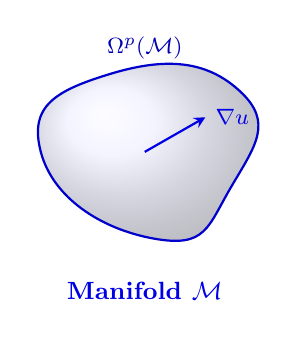
\begin{tikzpicture}[scale=1.1]
% --- CONTINUUM MANIFOLD (LEFT) ---
\begin{scope}[shift={(-3,0)}]
    \shade[ball color=blue!15, opacity=0.4] 
        plot [smooth cycle, tension=1] coordinates {(-1.2,0) (-0.4,0.9) (1.1,0.7) (1.0,-0.4) (0.1,-1)};
    \draw[thick, blue!80!black] 
        plot [smooth cycle, tension=1] coordinates {(-1.2,0) (-0.4,0.9) (1.1,0.7) (1.0,-0.4) (0.1,-1)};
    
    % Field representation
    \draw[->, >=stealth, blue!90!black, thick] (0,0) -- (0.7,0.4) node[right, font=\footnotesize] {$\nabla u$};
    
    \node[blue!90!black, font=\small\bfseries] at (0,-1.6) {Manifold $\mathcal{M}$};
    \node[blue!70!black, font=\footnotesize] at (0,1.2) {$\Omega^p(\mathcal{M})$};
\end{scope}
\end{tikzpicture}
\end{center}
\end{frame}

% ---------------- Slide 4 — The objects we will use ----------------
\begin{frame}{The combinatorial structure $\mathcal{M}$}

\begin{itemize}

\item We begin with a \textbf{finite cell complex} $\mathcal{M}$ as the primary “space” describing the relational structure of a physical system (no embedding required).
\vspace{0.2cm}

\item Cells represent entities of different dimension:
\begin{itemize}
\item vertices (0–cells)
\item edges (1–cells)
\item faces (2–cells)
\item higher–dimensional cells if needed
\end{itemize}
\vspace{0.2cm}

\item Physical quantities are represented as \textbf{combinatorial differential forms} (Forman):
a $k$–form assigns values to \emph{incident pairs} of cells $\sigma^{p} \prec \tau^{p+k}$.
\vspace{0.2cm}

\item These objects admit an \textbf{exterior derivative} defined through cell incidence.

\end{itemize}

\end{frame}

% ---------------- Slide 5 — From M to K (Forman subdivision) ----------------
\begin{frame}{The computational complex $\mathcal{K}$
\href{https://www.worldscientific.com/doi/abs/10.1142/S0129167X02001265}{\beamergotobutton{Forman 2002}}
}

\begin{itemize}

\item We assume $\mathcal{M}$ is built from \textbf{simple polytopes:} each vertex is incident to exactly $D$ $(D\!-\!1)$–cells.
\vspace{0.2cm}

\item We pass to its \textbf{Forman subdivision} $K$:
\begin{itemize}
\item vertices of $\mathcal{K}$ correspond to cells of $\mathcal{M}$,
\item adjacency reflects cell incidence in $\mathcal{M}$.
\end{itemize}
\vspace{0.2cm}

\item The resulting complex $\mathcal{K}$ is \textbf{quasi-cubical}: local neighborhoods resemble products of intervals.
\vspace{0.2cm}

\item Under this construction:
\begin{itemize}
    \item \textbf{combinatorial differential forms on $\mathcal{M}$ correspond naturally to cochains on $\mathcal{K}$.}
    \item \textbf{exterior derivatives of forms on $\mathcal{M}$ correspond naturally to coboundary operators of cochains on $\mathcal{K}$.}
    \item the quasi-cubical structure enables a \textbf{natural cup product on cochains}.
\end{itemize}
\vspace{0.2cm}

\end{itemize}
\end{frame}


\begin{frame}{Chains and cochains}
\begin{itemize}
\vspace{0.5cm}
\item $C_p(\mathcal{K})$: formal linear combinations of oriented $p$-cells.
\vspace{0.5cm}
\item $C^p(\mathcal{K})$: linear functionals on $C_p(\mathcal{K})$.
\end{itemize}
\vspace{0.5cm}

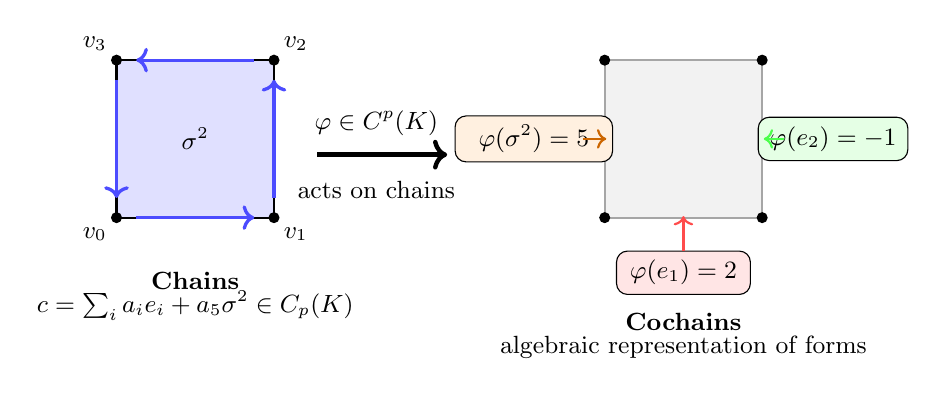
\begin{tikzpicture}[scale=1.0, every node/.style={font=\small}]
\centering

% --- Left: quasi-cubical cell complex / chains ---
\begin{scope}[shift={(-4.2, 0)}]
    % square face
    \fill[blue!12] (0,0) rectangle (2,2);
    \draw[thick] (0,0) rectangle (2,2);

    % oriented edges
    \draw[->, very thick, blue!70] (0.25,0) -- (1.75,0);     % bottom
    \draw[->, very thick, blue!70] (2,0.25) -- (2,1.75);     % right
    \draw[->, very thick, blue!70] (1.75,2) -- (0.25,2);     % top
    \draw[->, very thick, blue!70] (0,1.75) -- (0,0.25);     % left

    % vertices
    \fill (0,0) circle (2pt) node[below left] {$v_0$};
    \fill (2,0) circle (2pt) node[below right] {$v_1$};
    \fill (2,2) circle (2pt) node[above right] {$v_2$};
    \fill (0,2) circle (2pt) node[above left] {$v_3$};

    % face label
    \node at (1,1) {$\sigma^2$};

    % caption
    \node[align=center] at (1,-1.0) {\textbf{Chains} \\[-1mm] $c=\sum_i a_i e_i + a_5 \sigma^2 \in C_p(K)$};
\end{scope}

% --- Middle: dual arrow ---
\draw[->, ultra thick] (-1.65, 0.8) -- (0.0, 0.8);
\node at (-0.9, 1.2) {$\varphi \in C^p(K)$};
\node at (-0.9, 0.35) {\small acts on chains};

% --- Right: cochains / functionals ---
\begin{scope}[shift={(2.0, 0)}]
    % same quasi-cubical complex faintly
    \fill[gray!10] (0,0) rectangle (2,2);
    \draw[thick, gray!70] (0,0) rectangle (2,2);
    \fill (0,0) circle (2pt);
    \fill (2,0) circle (2pt);
    \fill (2,2) circle (2pt);
    \fill (0,2) circle (2pt);

    % highlighted evaluations
    \node[draw, rounded corners, fill=red!10, minimum width=1.7cm, minimum height=0.55cm] at (1,-0.7) {$\varphi(e_1)=2$};
    \node[draw, rounded corners, fill=green!10, minimum width=1.9cm, minimum height=0.55cm] at (2.9,1.0) {$\varphi(e_2)=-1$};
    \node[draw, rounded corners, fill=orange!12, minimum width=2.0cm, minimum height=0.55cm] at (-0.9,1.0) {$\varphi(\sigma^2)=5$};

    \draw[->, thick, red!70] (1,-0.42) -- (1,0.02);
    \draw[->, thick, green!70] (2.28,1.0) -- (2.02,1.0);
    \draw[->, thick, orange!80!black] (-0.28,1.0) -- (0.02,1.0);

    % caption
    \node[align=center] at (1,-1.5) {\textbf{Cochains} \\[-1mm] algebraic representation of forms};
\end{scope}

\end{tikzpicture}
\end{frame}

\begin{frame}{Cup product on cochains}

\begin{itemize}

\item The cochain spaces \(C^\bullet(\mathcal{K})\) carry a graded product
\[
\smile \;:\; C^p(\mathcal{K}) \times C^q(\mathcal{K}) \longrightarrow C^{p+q}(\mathcal{K}),
\]
called the \textbf{cup product}. \href{https://www.sciencedirect.com/science/article/pii/S0307904X22002657\#bib0023}{\beamergotobutton{Berbatov 2022}}

\vspace{0.2cm}

\item Under the correspondence between combinatorial differential forms on \(\mathcal{M}\) and cochains on \(\mathcal{K}\), the cup product is the algebraic counterpart of the \textbf{exterior (wedge) product} of forms.

\vspace{0.2cm}

\item This is needed later for
\textbf{higher-order algebraic constructions},
including constitutive couplings, vector-valued operations, and bracket-type structures.

\vspace{0.2cm}

\item NOTE: Unlike the smooth wedge product, the cup product is in general \textbf{not associative}.

\end{itemize}

\end{frame}

\begin{frame}{Boundary and coboundary operators}
\begin{itemize}

\item Boundary operator on chains:
\[
\partial : C_{p+1}(\mathcal{K}) \rightarrow C_p(\mathcal{K})
\]

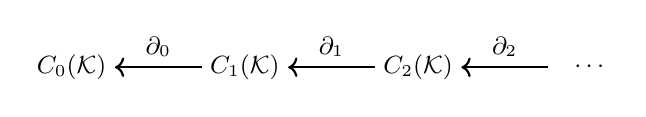
\begin{tikzpicture}[scale=1.0, every node/.style={font=\small}]
\centering
\begin{scope}[shift={(-2.3, -2.8)}]
    \node (c0) at (0,0) {$C_0(\mathcal{K})$};
    \node (c1) at (2.2,0) {$C_1(\mathcal{K})$};
    \node (c2) at (4.4,0) {$C_2(\mathcal{K})$};
    \node (c3) at (6.6,0) {$\cdots$};

    \draw[<-, thick] (0.55,0) -- (1.65,0) node[midway, above] {$\partial_0$};
    \draw[<-, thick] (2.75,0) -- (3.85,0) node[midway, above] {$\partial_1$};
    \draw[<-, thick] (4.95,0) -- (6.05,0) node[midway, above] {$\partial_2$};
\end{scope}
\end{tikzpicture}

\begin{itemize}
    \item $C_\bullet(\mathcal{K})$ is a chain complex: $\partial^2=0$.
\end{itemize}
\vspace{0.5cm}

\item Coboundary operator on cochains:
\[
\delta : C^p(\mathcal{K}) \rightarrow C^{p+1}(\mathcal{K})
\]
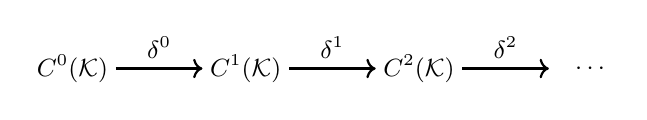
\begin{tikzpicture}[scale=1.0, every node/.style={font=\small}]
\centering
\begin{scope}[shift={(-2.3, -2.8)}]
    \node (c0) at (0,0) {$C^0(\mathcal{K})$};
    \node (c1) at (2.2,0) {$C^1(\mathcal{K})$};
    \node (c2) at (4.4,0) {$C^2(\mathcal{K})$};
    \node (c3) at (6.6,0) {$\cdots$};

    \draw[->, thick] (0.55,0) -- (1.65,0) node[midway, above] {$\delta^0$};
    \draw[->, thick] (2.75,0) -- (3.85,0) node[midway, above] {$\delta^1$};
    \draw[->, thick] (4.95,0) -- (6.05,0) node[midway, above] {$\delta^2$};
\end{scope}
\end{tikzpicture}
\begin{itemize}
    \item $C^\bullet(\mathcal{K})$ is a cochain complex: $\delta^2=0$.
\end{itemize}
\end{itemize}

\end{frame}


\begin{frame}{Discrete Stokes theorem}

\begin{itemize}

\item Combinatorial analogue of
\textbf{Stokes' theorem}:
\[
\langle \delta \varphi , c \rangle
=
\langle \varphi , \partial c \rangle
\]
\item Boundary/coboundary are dual: “integration by parts” is algebraic.
\item Conservation and compatibility become identities in the cochain complex.
\item This is the structural reason cochains are the right level of abstraction for transport.
\end{itemize}

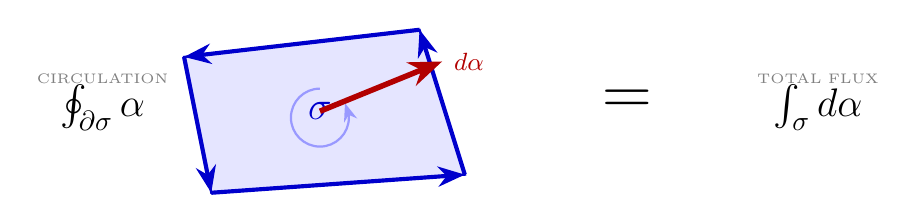
\begin{tikzpicture}[x=1cm, y=1cm, >=Stealth, scale=1.15]

  % ---------- Styling ----------
  \tikzset{
    face/.style={fill=blue!10, draw=blue!80!black, line width=0.8pt},
    edge/.style={draw=blue!80!black, line width=1.5pt, ->},
    flux/.style={draw=red!70!black, line width=2pt, ->},
    labelstyle/.style={font=\sffamily\small\bfseries}
  }

  % ---------- Geometry: Quasi-cubical face ----------
  \coordinate (A) at (0,0);
  \coordinate (B) at (2.8,0.2);
  \coordinate (C) at (2.3,1.8);
  \coordinate (D) at (-0.3,1.5);
  \coordinate (Center) at (1.2,0.9);

  % ---------- The Face (Interior) ----------
  \filldraw[face] (A) -- (B) -- (C) -- (D) -- cycle;

  % Orientation indicator
  \draw[->, blue!40, thick] (1.2,1.15) arc[start angle=90,end angle=390,radius=0.32];
  \node[blue!80!black, font=\Large\bfseries] at (Center) {$\sigma$};

  % ---------- Boundary Edges ----------
  \draw[edge] (A) -- (B);
  \draw[edge] (B) -- (C);
  \draw[edge] (C) -- (D);
  \draw[edge] (D) -- (A);

  % ---------- Exterior Derivative / Flux ----------
  \draw[flux] (Center) -- ++(1.35,0.55)
    node[right, labelstyle, color=red!70!black] {$d\alpha$};

  % ---------- Visual Duality Equation ----------
  \node[align=center] at (-1.2,1) {
    \color{gray}\tiny CIRCULATION\\
    \Large $\oint_{\partial\sigma} \alpha$
  };

  \node at (4.6,1) {\Huge $=$};

  \node[align=center] at (6.7,1) {
    \color{gray}\tiny TOTAL FLUX\\
    \Large $\int_{\sigma} d\alpha$
  };

\end{tikzpicture}
\end{frame}

% ---------------- Slide 8 — Relation to DEC/FEEC (NEW; crucial) ----------------
\begin{frame}{Relation to discrete exterior calculus and FEEC}
\begin{itemize}
\item \textbf{Shared:} cochains, coboundary.
\vspace{0.3cm}
\item \textbf{Different emphasis:} not a discretisation of a given manifold; $\mathcal{K}$ is primary and may evolve.
\vspace{0.3cm}
\item \textbf{Different challenge:} vector-valued quantities with \emph{non-uniform fibres} and transport as extra structure.
\end{itemize}
\vspace{0.3cm}

\usetikzlibrary{arrows.meta, shapes.geometric, backgrounds}

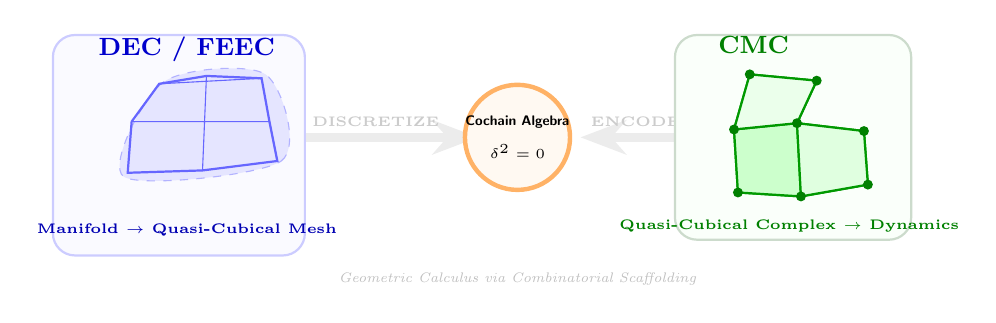
\begin{tikzpicture}[x=1cm, y=1cm, >=Stealth, scale=1.0, font=\sffamily]

  % ---------- Background Connections (Drawn First) ----------
  \draw[->, line width=3pt, gray!15] (-2.9, 0) -- (-0.5, 0);
  \draw[->, line width=3pt, gray!15] (2.2, 0) -- (0.8, 0);
  
  \node[gray!40, font=\tiny\bfseries] at (-1.8, 0.2) {DISCRETIZE};
  \node[gray!40, font=\tiny\bfseries] at (1.5, 0.2) {ENCODE};

  % ---------- DEC / FEEC (Left: Top-Down) ----------
  \begin{scope}[shift={(-4, 0)}]
    \draw[blue!20, fill=blue!2, rounded corners=8pt, thick] (-1.9,-1.5) rectangle (1.3, 1.3);
    \node[anchor=north, blue!80!black, font=\small\bfseries] at (-0.2, 1.4) {DEC / FEEC};
    
    % Smooth vs quasi-cubical mesh visual
    \fill[blue!10] plot[smooth cycle] coordinates {(-1,-0.5) (1,-0.3) (0.8,0.8) (-0.5,0.7)};
    \draw[blue!30, dashed] plot[smooth cycle] coordinates {(-1,-0.5) (1,-0.3) (0.8,0.8) (-0.5,0.7)};
    
    % Quasi-cubical mesh
    \draw[blue!60, thick]
      (-0.95,-0.45) -- (0.00,-0.42) -- (0.95,-0.30)
      -- (0.85,0.20) -- (0.75,0.75) -- (0.05,0.78)
      -- (-0.55,0.68) -- (-0.90,0.20) -- cycle;
    \draw[blue!60, thin]
      (0.00,-0.42) -- (0.05,0.78)
      (-0.55,0.68) -- (0.75,0.75)
      (-0.90,0.20) -- (0.85,0.20);
    
    \node[below=5pt, blue!70!black, font=\tiny\bfseries] at (-0.2,-0.8) {Manifold $\to$ Quasi-Cubical Mesh};
  \end{scope}

  % ---------- CMC (Right: Bottom-Up) ----------
  \begin{scope}[shift={(3.8, 0)}]
    \draw[green!30!black!20, fill=green!2, rounded corners=8pt, thick] (-1.8, -1.3) rectangle (1.2, 1.3);
    \node[anchor=north, green!50!black, font=\small\bfseries] at (-0.8, 1.4) {CMC};
    
    % Abstract quasi-cubical complex
    \coordinate (a) at (-1.00,-0.70);
    \coordinate (b) at (-0.20,-0.75);
    \coordinate (c) at (0.65,-0.60);
    \coordinate (d) at (-1.05,0.10);
    \coordinate (e) at (-0.25,0.18);
    \coordinate (f) at (0.60,0.08);
    \coordinate (g) at (-0.85,0.80);
    \coordinate (h) at (0.00,0.72);
    
    % 1-skeleton of a quasi-cubical complex
    \draw[green!60!black, thick]
      (a)--(b)--(c)
      (d)--(e)--(f)
      (g)--(h)
      (a)--(d)--(g)
      (b)--(e)--(h)
      (c)--(f);
    
    % emphasize quadrilateral 2-cells
    \filldraw[fill=green!20, draw=green!60!black, thick] (a)--(b)--(e)--(d)--cycle;
    \filldraw[fill=green!12, draw=green!60!black, thick] (b)--(c)--(f)--(e)--cycle;
    \filldraw[fill=green!8,  draw=green!60!black, thick] (d)--(e)--(h)--(g)--cycle;
    
    \foreach \p in {a,b,c,d,e,f,g,h} \fill[green!50!black] (\p) circle (1.8pt);
    
    \node[below=5pt, green!50!black, font=\tiny\bfseries] at (-0.35, -0.75) {Quasi-Cubical Complex $\to$ Dynamics};
  \end{scope}

  % ---------- Shared Core (Middle: Drawn Last) ----------
  \node[draw = orange!60, fill=orange!5, circle, ultra thick, inner sep=-1pt, align=center] (core) at (0, 0) {
    \textbf{\tiny Cochain Algebra}\\
    \tiny $\delta^2 = 0$
  };

  % ---------- Footer ----------
  \node[gray!50, font=\tiny\itshape] at (0,-1.8) {Geometric Calculus via Combinatorial Scaffolding};

\end{tikzpicture}
\end{frame}

\begin{frame}{Scalar quantities on the complex}
\begin{itemize}
\item Extensive quantities attach naturally to top-dimensional cells (or chosen $p$-cells).
\item Fluxes attach to codimension-one cells (interfaces), consistent with incidence.
\item Balance laws are expressed using coboundary: \textbf{outflow is a coboundary of flux}.
\end{itemize}
% Keep the “two cells share an interface” picture; remove the algebraic box with full sums.


\centering
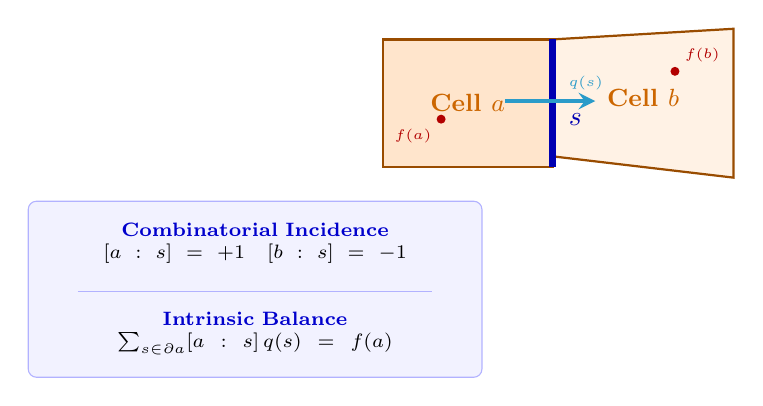
\begin{tikzpicture}[scale=1.35, every node/.style={font=\scriptsize}]

% --- GEOMETRY (Top Section): quasi-cubical example ---
\begin{scope}
    % Coordinates
    \coordinate (A) at (0,0);
    \coordinate (B) at (1.6,0);
    \coordinate (C) at (1.6,1.2);
    \coordinate (D) at (0,1.2);

    \coordinate (E) at (1.6,0.1);
    \coordinate (F) at (3.3,-0.1);
    \coordinate (G) at (3.3,1.3);
    \coordinate (H) at (1.6,1.2);

    % 2-cells (Faces)
    \fill[orange!20, draw=orange!60!black, thick] (A)--(B)--(C)--(D)--cycle;
    \fill[orange!10, draw=orange!60!black, thick] (E)--(F)--(G)--(H)--cycle;
    
    \node[orange!80!black, font=\bfseries] at (0.8,0.6) {\small Cell $a$};
    \node[orange!80!black, font=\bfseries] at (2.45,0.65) {\small Cell $b$};

    % Shared interface (1-cell)
    \draw[line width=2.5pt, blue!70!black] (B)--(C);
    \node[blue!70!black, font=\bfseries, anchor=west] at (1.66, 0.45) {$s$};

    % Flux arrow (oriented interface measurement)
    \draw[->, ultra thick, cyan!80!black, >=stealth] (1.15,0.62) -- (2.0,0.62)
        node[midway, above, font=\tiny\bfseries] {\ \ \ \ \ \ \ \ \ \ $q(s)$};

    % Local sources / potentials
    \fill[red!70!black] (0.55,0.45) circle (1.2pt) node[below left, font=\tiny] {$f(a)$};
    \fill[red!70!black] (2.75,0.9) circle (1.2pt) node[above right, font=\tiny] {$f(b)$};
\end{scope}

% --- ALGEBRAIC LOGIC (Bottom Section) ---
\begin{scope}[shift={(-1.2, -1.15)}]
    \node[draw=blue!30, fill=blue!5, rounded corners=3pt, inner sep=8pt, align=center, text width=5.2cm] (box) {
        {\color{blue!80!black}\textbf{Combinatorial Incidence}}\\
        $[a:s] = +1 \quad [b:s] = -1$\\[4pt]
        \makebox[4.5cm]{\color{blue!30}\rule{4.5cm}{0.4pt}}\\[4pt]
        {\color{blue!80!black}\textbf{Intrinsic Balance}}\\
        $\sum_{s \in \partial a} [a:s]\,q(s) = f(a)$
    };
\end{scope}

\end{tikzpicture}
\end{frame}

% ---------------- Slide 11a — Metric and Constitutive Structure ----------------
\begin{frame}{Metric and Constitutive Structure}
\begin{columns}[T,onlytextwidth]

% ================= LEFT =================
\column{0.60\textwidth}
\vspace{-0.7cm}
\begin{block}{\small Metric is introduced \emph{after} topology}
\begin{itemize}
\item \textbf{Topology:} incidence $\Rightarrow$ $\partial,\delta$
\item \textbf{Metric:} assign measures to cells, then define inner products
\item \textbf{Geometry:} constitutive maps use the metric layer
\end{itemize}
\end{block}

\begin{block}{\small Inner products on cochain spaces}
\begin{itemize}
\item \textbf{Cell measures (weights):} choose \(\mu_p:\mathcal{K}_p\to\mathbb{R}^+\).
\item \textbf{Inner product} on $C^p(\mathcal{K})$ defined for given $\mu_p$.
\item \textbf{Adjoint coboundary} $\delta^\star:C^{p+1}(\mathcal{K})\to C^p(\mathcal{K}$ defined by
\vspace{-0.8cm}
\[
\langle \delta\sigma,\tau\rangle_{p+1} \;=\; \langle \sigma,\delta^\star\tau\rangle_p .
\]
\end{itemize}
\end{block}

% ================= RIGHT =================
\column{0.38\textwidth}
\begin{center}
\vspace{-0.8cm}
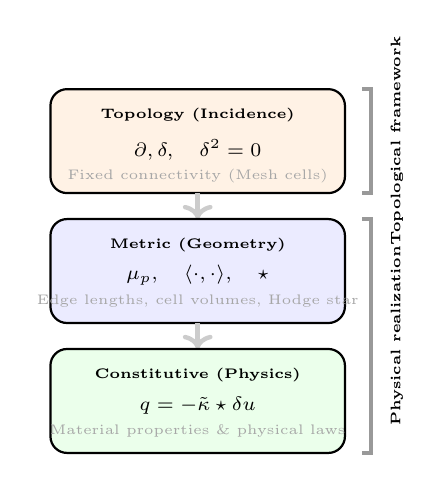
\begin{tikzpicture}[scale=1.1, every node/.style={font=\scriptsize}]

% Layer 1: Topology
\draw[rounded corners=6pt, thick, fill=orange!10] (-1.7, 1.2) rectangle (1.7, 2.4);
\node[font=\bfseries\tiny] at (0, 2.1) {Topology (Incidence)};
\node at (0, 1.7) {\(\partial, \delta, \quad \delta^2=0\)};
\node[gray!70] at (0, 1.4) {\tiny Fixed connectivity (Mesh cells)};

% Connection Arrow 1
\draw[->, ultra thick, gray!40] (0, 1.2) -- (0, 0.9);

% Layer 2: Metric
\draw[rounded corners=6pt, thick, fill=blue!8] (-1.7, -0.3) rectangle (1.7, 0.9);
\node[font=\bfseries\tiny] at (0, 0.6) {Metric (Geometry)};
\node at (0, 0.25) {\(\mu_p, \quad \langle\cdot,\cdot\rangle, \quad \star\)};
\node[gray!70] at (0, -0.05) {\tiny Edge lengths, cell volumes, Hodge star};

% Connection Arrow 2
\draw[->, ultra thick, gray!40] (0, -0.3) -- (0, -0.6);

% Layer 3: Constitutive
\draw[rounded corners=6pt, thick, fill=green!8] (-1.7, -1.8) rectangle (1.7, -0.6);
\node[font=\bfseries\tiny] at (0, -0.9) {Constitutive (Physics)};
\node at (0, -1.25) {\(q = -\tilde{\kappa} \star \delta u\)};
\node[gray!70] at (0, -1.55) {\tiny Material properties \& physical laws};

% Right side brackets with vertical text
\draw[very thick, gray!80] (1.9, 2.4) -- (2.0, 2.4) -- (2.0, 1.2) -- (1.9, 1.2);
\node[anchor=center, font=\bfseries\tiny, rotate=90] at (2.3, 1.8) {Topological framework};

\draw[very thick, gray!80] (1.9, 0.9) -- (2.0, 0.9) -- (2.0, -1.8) -- (1.9, -1.8);
\node[anchor=center, font=\bfseries\tiny, rotate=90] at (2.3, -0.45) {Physical realization};

\end{tikzpicture}
\end{center}

\end{columns}
\end{frame}

% ---------------- Slide 13 — Applications of Scalar Framework ----------------
\begin{frame}{Applications of the scalar framework
\href{https://arxiv.org/abs/2505.09443}{\beamergotobutton{Berbatov 2025}}
}

\begin{columns}[T,onlytextwidth]

% ---------------- LEFT: TEXT ----------------
\column{0.67\textwidth}
\vspace{-0.50cm}
\begin{block}{\small Strong, primal weak and mixed weak formulations developed, and used for}
\begin{enumerate}
\item \textbf{\small Diffusion on heterogeneous complexes}\\[-2pt]
{\scriptsize mass diffusion / heat conduction / charge transport on irregular cells}
\item \textbf{\small Flow in porous and fractured media}\\[-2pt]
{\scriptsize flux through \((D\!-\!1)\)-cells; interfaces model cracks and pores}
\href{https://www.sciencedirect.com/science/article/pii/S030917082500209X}{\beamergotobutton{Liu 2025}}
\href{https://www.sciencedirect.com/science/article/pii/S1365160926000365}{\beamergotobutton{Liu 2026}}
\item \textbf{\small Coupled thermo--chemical transport}\\[-2pt]
{\scriptsize multiple scalar species + reaction/production terms on \(D\)-cells}
\item \textbf{\small Variational initial--boundary problems}\\[-2pt]
{\scriptsize primal \& mixed forms; efficient solves via diagonal stiffness in the mixed form}
\end{enumerate}
\end{block}

% ---------------- RIGHT: FIGURE ----------------
\column{0.40\textwidth}
\begin{center}
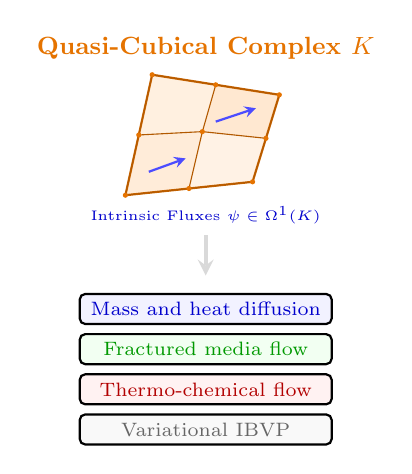
\begin{tikzpicture}[scale=0.85, every node/.style={font=\scriptsize}]

% --- TOP SECTION: THE MESH COMPLEX ---
\begin{scope}
    % Quasi-cubical / quasi-quadrilateral complex
    \coordinate (P1) at (0,0);
    \coordinate (P2) at (1.9,0.2);
    \coordinate (P3) at (2.3,1.5);
    \coordinate (P4) at (0.4,1.8);

    % Mid-edge / irregular subdivision points
    \coordinate (M12) at (0.95,0.10);
    \coordinate (M23) at (2.10,0.85);
    \coordinate (M34) at (1.35,1.65);
    \coordinate (M41) at (0.20,0.90);
    \coordinate (C)   at (1.15,0.95);

    % Quasi-cubical 2-cells (irregular quadrilateral faces)
    \fill[orange!15] (P1)--(M12)--(C)--(M41)--cycle;
    \fill[orange!10] (M12)--(P2)--(M23)--(C)--cycle;
    \fill[orange!18] (C)--(M23)--(P3)--(M34)--cycle;
    \fill[orange!12] (M41)--(C)--(M34)--(P4)--cycle;

    % Outer boundary
    \draw[thick, orange!80!black] (P1)--(P2)--(P3)--(P4)--cycle;

    % Internal incidence structure
    \draw[orange!70!black]
        (M12)--(C)--(M34)
        (M41)--(C)--(M23)
        (P1)--(M12) (M12)--(P2)
        (P2)--(M23) (M23)--(P3)
        (P3)--(M34) (M34)--(P4)
        (P4)--(M41) (M41)--(P1);

    % Nodes
    \foreach \p in {P1,P2,P3,P4,M12,M23,M34,M41,C}
        \fill[orange!90!black] (\p) circle (1.1pt);

    % Flow/Flux intrinsic representation
    \draw[thick, ->, >=stealth, blue!70] (0.35,0.35) -- (0.90,0.55);
    \draw[thick, ->, >=stealth, blue!70] (1.35,1.10) -- (1.95,1.30);

    \node[orange!90!black, font=\bfseries] at (1.2, 2.2) {\small Quasi-Cubical Complex $K$};
    \node[blue!80!black, font=\tiny] at (1.2, -0.3) {Intrinsic Fluxes $\psi \in \Omega^1(K)$};
\end{scope}

% --- TRANSITION ARROW ---
\draw[->, >=stealth, line width=1.5pt, gray!30] (1.2,-0.6) -- (1.2,-1.2);

% --- BOTTOM SECTION: APPLICATION BADGES (Narrowed for columns) ---
\begin{scope}[shift={(1.2,-1.7)}]
    \node[draw, thick, rounded corners=2pt, fill=blue!5, text=blue!80!black, inner sep=3pt, minimum width=3.2cm] (B1) at (0,0) 
        {Mass and heat diffusion};
    \node[draw, thick, rounded corners=2pt, fill=green!5, text=green!60!black, inner sep=3pt, minimum width=3.2cm] (B2) at (0,-0.6) 
        {Fractured media flow};
    \node[draw, thick, rounded corners=2pt, fill=red!5, text=red!70!black, inner sep=3pt, minimum width=3.2cm] (B3) at (0,-1.2) 
        {Thermo-chemical flow};
    \node[draw, thick, rounded corners=2pt, fill=gray!5, text=gray!80!black, inner sep=3pt, minimum width=3.2cm] (B4) at (0,-1.8) 
        {Variational IBVP};
\end{scope}

\end{tikzpicture}
\end{center}

\end{columns}
\end{frame}

% ---------------- Slide 14 — Why scalars are insufficient (keep concise) ----------------
\begin{frame}{Scalars are not sufficient}
\begin{itemize}
\item Mechanics requires vector/covector-type quantities (forces, momenta, displacements).
\item In a combinatorial setting there is no ambient tangent bundle by default.
\item Therefore vectors must live in \textbf{fibres} attached to cells/vertices; transport is additional structure.
\end{itemize}



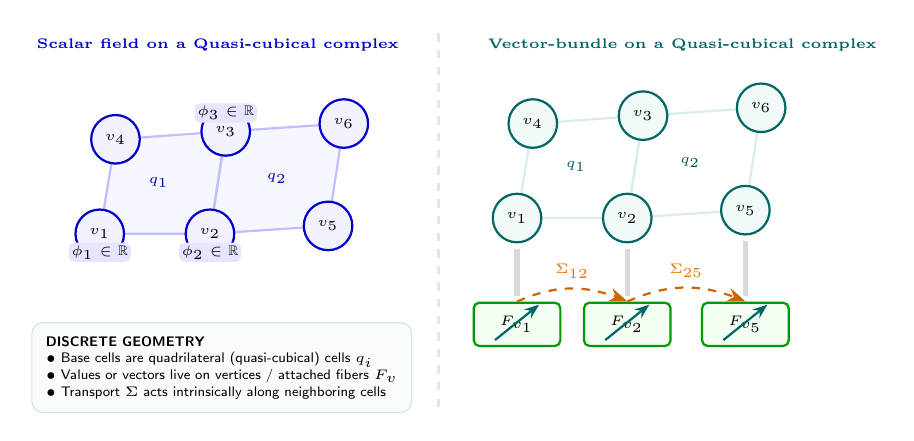
\begin{tikzpicture}[
    scale=1.0,
    >=Stealth,
    cell/.style={circle, draw=blue!80!black, thick, minimum size=5.8mm, fill=blue!5, font=\sffamily\tiny\bfseries},
    vcell/.style={circle, draw=teal!80!black, thick, minimum size=5.8mm, fill=teal!5, font=\sffamily\tiny\bfseries},
    fiber/.style={draw=green!60!black, thick, fill=green!5, rounded corners=2pt, minimum width=1.1cm, minimum height=0.55cm, font=\sffamily\tiny},
    vec/.style={->, thick, teal!80!black, >={Stealth[scale=0.8]}},
    trans/.style={->, dashed, thick, orange!80!black, >={Stealth[bend]}},
    title/.style={font=\sffamily\footnotesize\bfseries}
]

% --- Left Section: Scalar field on a quasi-cubical complex ---
\node[title, blue!80!black, font=\tiny\bfseries] at (-2.7, 3.0) {Scalar field on a Quasi-cubical complex};

% Vertices of two adjacent quadrilateral cells
\coordinate (A) at (-4.2, 0.6);
\coordinate (B) at (-2.8, 0.6);
\coordinate (C) at (-2.6, 1.9);
\coordinate (D) at (-4.0, 1.8);

\coordinate (E) at (-1.3, 0.7);
\coordinate (F) at (-1.1, 2.0);

% Filled quasi-cubical cells
\fill[blue!5, opacity=0.6] (A) -- (B) -- (C) -- (D) -- cycle;
\fill[blue!8, opacity=0.45] (B) -- (E) -- (F) -- (C) -- cycle;

\draw[thick, blue!25] (A) -- (B) -- (C) -- (D) -- cycle;
\draw[thick, blue!25] (B) -- (E) -- (F) -- (C) -- cycle;

% Vertex nodes
\node[cell] (s1) at (A) {$v_1$};
\node[cell] (s2) at (B) {$v_2$};
\node[cell] (s3) at (C) {$v_3$};
\node[cell] (s4) at (D) {$v_4$};
\node[cell] (s5) at (E) {$v_5$};
\node[cell] (s6) at (F) {$v_6$};

% Example scalar values
\node[fill=blue!10, rounded corners=2pt, inner sep=1pt, font=\tiny\bfseries, below=3pt] at (s1) {$\phi_1 \in \mathbb{R}$};
\node[fill=blue!10, rounded corners=2pt, inner sep=1pt, font=\tiny\bfseries, below=3pt] at (s2) {$\phi_2 \in \mathbb{R}$};
\node[fill=blue!10, rounded corners=2pt, inner sep=1pt, font=\tiny\bfseries, above=3pt] at (s3) {$\phi_3 \in \mathbb{R}$};

% Cell labels
\node[font=\sffamily\tiny\bfseries, blue!70!black] at (-3.45, 1.25) {$q_1$};
\node[font=\sffamily\tiny\bfseries, blue!70!black] at (-1.95, 1.3) {$q_2$};

% --- Divider ---
\draw[lightgray!40, line width=1pt, dashed] (0.1, -1.6) -- (0.1, 3.2);

% --- Right Section: Vector bundle on the same quasi-cubical complex ---
\node[title, teal!80!black, font=\tiny\bfseries] at (3.2, 3.0) {Vector-bundle on a Quasi-cubical complex};

% Same combinatorial pattern, shifted right
\coordinate (VA) at (1.1, 0.8);
\coordinate (VB) at (2.5, 0.8);
\coordinate (VC) at (2.7, 2.1);
\coordinate (VD) at (1.3, 2.0);

\coordinate (VE) at (4.0, 0.9);
\coordinate (VF) at (4.2, 2.2);

\draw[thick, teal!15] (VA) -- (VB) -- (VC) -- (VD) -- cycle;
\draw[thick, teal!15] (VB) -- (VE) -- (VF) -- (VC) -- cycle;

\node[vcell] (v1) at (VA) {$v_1$};
\node[vcell] (v2) at (VB) {$v_2$};
\node[vcell] (v3) at (VC) {$v_3$};
\node[vcell] (v4) at (VD) {$v_4$};
\node[vcell] (v5) at (VE) {$v_5$};
\node[vcell] (v6) at (VF) {$v_6$};

% Fibers attached to selected vertices
\node[fiber] (f1) at (1.1, -0.55) {$F_{v_1}$};
\node[fiber] (f2) at (2.5, -0.55) {$F_{v_2}$};
\node[fiber] (f3) at (4.0, -0.55) {$F_{v_5}$};

% Attachments
\draw[draw=gray!30, line width=2pt, shorten >=2pt, shorten <=2pt] (v1) -- (f1);
\draw[draw=gray!30, line width=2pt, shorten >=2pt, shorten <=2pt] (v2) -- (f2);
\draw[draw=gray!30, line width=2pt, shorten >=2pt, shorten <=2pt] (v5) -- (f3);

% Internal vectors
\draw[vec] (0.82, -0.75) -- (1.38, -0.3);
\draw[vec] (2.22, -0.75) -- (2.78, -0.3);
\draw[vec] (3.72, -0.75) -- (4.28, -0.3);

% Parallel transport along edges of the quasi-cubical complex
\draw[trans, bend left=24] (f1.north) to node[midway, above, font=\tiny\bfseries, orange!90!black] {$\Sigma_{12}$} (f2.north);
\draw[trans, bend left=24] (f2.north) to node[midway, above, font=\tiny\bfseries, orange!90!black] {$\Sigma_{25}$} (f3.north);

% Cell labels
\node[font=\sffamily\tiny\bfseries, teal!70!black] at (1.85, 1.45) {$q_1$};
\node[font=\sffamily\tiny\bfseries, teal!70!black] at (3.3, 1.5) {$q_2$};

% --- Legend / Bottom Logic ---
\begin{scope}[shift={(-2.65, -1.1)}]
    \node[draw=teal!20, fill=teal!2, rounded corners=4pt, inner sep=5pt, font=\sffamily\tiny, align=left] {
        \textbf{DISCRETE GEOMETRY}\\
        $\bullet$ Base cells are quadrilateral (quasi-cubical) cells $q_i$\\
        $\bullet$ Values or vectors live on vertices / attached fibers $F_v$\\
        $\bullet$ Transport $\Sigma$ acts intrinsically along neighboring cells
    };
\end{scope}

\end{tikzpicture}
\end{frame}

% ---------------- Slide 15 — Fibres with varying rank (keep; reframe as bundle over 0-skeleton) ----------------
\begin{frame}{A bundle over the 0-skeleton (with varying fibre rank)}
\begin{itemize}
\item Attach a vector space $F_v$ to each vertex $v$ (a “bundle” over $\mathcal{K}_0$).
\item $F_v$ is generated by edges incident to $v$ (star of $v$).
\item \textbf{Key difficulty:} $\dim F_v$ varies with valence; there is no canonical identification $F_v \cong F_w$.
\end{itemize}

\centering
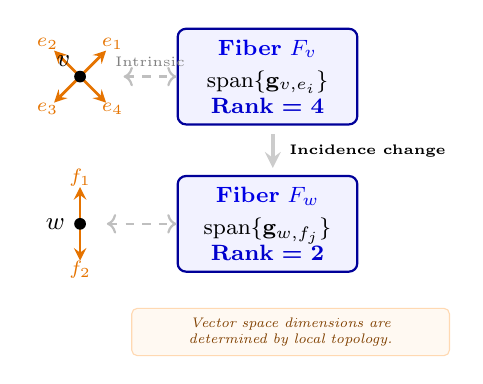
\begin{tikzpicture}[
  scale=0.85,
  every node/.style={font=\footnotesize},
  fibbox/.style={rectangle, rounded corners=3pt, line width=0.8pt, fill=blue!5,
    draw=blue!60!black, inner sep=4pt, text width=2.0cm, align=center},
  ray/.style={line width=1.0pt, ->, orange!90!black, >=stealth},
  dot/.style={fill=black, circle, inner sep=1.5pt}
]

% ====== TOP SECTION: High Connectivity ======
\begin{scope}[local bounding box=Top]
    \coordinate (v) at (0,0);
    \foreach \ang/\name in {45/e_1, 135/e_2, 225/e_3, 315/e_4}{
      \draw[ray] (v) -- ++(\ang:0.55)
        node[pos=1.25, font=\scriptsize\bfseries] {$\name$};
    }
    \node[dot] at (v) {};
    \node[anchor=south east, font=\small\bfseries] at (v) {$v$};

    \node[fibbox] (boxV) at (2.8,0) {
        {\footnotesize\bfseries\color{blue!90!black} Fiber $F_v$} \\[2pt]
        $\mathrm{span}\{\mathbf{g}_{v,e_i}\}$ \\
        \textcolor{blue!80!black}{\textbf{Rank = 4}}
    };

    \draw[<->, thick, dashed, gray!50] (0.65,0) -- (boxV.west)
        node[midway, above, font=\tiny, text=gray] {Intrinsic};
\end{scope}

% ====== VERTICAL TRANSITION ======
\draw[->, line width=1.5pt, gray!40, >=stealth]
    ($(Top.south)+(1.2,-0.15)$) -- ($(Top.south)+(1.2,-0.65)$)
    node[midway, right=2pt, text=black, font=\tiny\bfseries] {Incidence change};

% ====== BOTTOM SECTION: Low Connectivity ======
\begin{scope}[shift={(0,-2.2)}, local bounding box=Bottom]
    \coordinate (w) at (0,0);
    \foreach \ang/\name in {90/1, 270/2}{
      \draw[ray] (w) -- ++(\ang:0.55)
        node[pos=1.25, font=\scriptsize\bfseries] {$f_{\name}$};
    }
    \node[dot] at (w) {};
    \node[anchor=east, font=\small\bfseries, xshift=-2pt] at (w) {$w$};

    \node[fibbox] (boxW) at (2.8,0) {
        {\footnotesize\bfseries\color{blue!90!black} Fiber $F_w$} \\[2pt]
        $\mathrm{span}\{\mathbf{g}_{w,f_j}\}$ \\
        \textcolor{blue!80!black}{\textbf{Rank = 2}}
    };

    \draw[<->, thick, dashed, gray!50] (0.4,0) -- (boxW.west);
\end{scope}

% ====== GLOBAL ANNOTATION ======
\node[draw=orange!30, fill=orange!5, rounded corners=2pt,
    font=\tiny\itshape, text=orange!50!black,
    anchor=north, text width=3.8cm, align=center]
    at ($(Bottom.south)+(1.4,-0.3)$)
    {Vector space dimensions are determined by local topology.};

\end{tikzpicture}

\end{frame}

% ---------------- Slide 16 — Vector-valued 0-forms (simplify) ----------------
\begin{frame}{Vector-valued 0-forms as sections}
\begin{itemize}
\item A vector field is a choice of element $u(v)\in F_v$ at each vertex.
\item Comparing $u(v)$ and $u(w)$ requires a transport rule (not automatic).
\item This is the point where “connection-like” structure becomes necessary.
\end{itemize}
% Drop the “non-canonical marker” box and the big layered diagram; keep one simple edge with $F_v, F_w$.

\centering
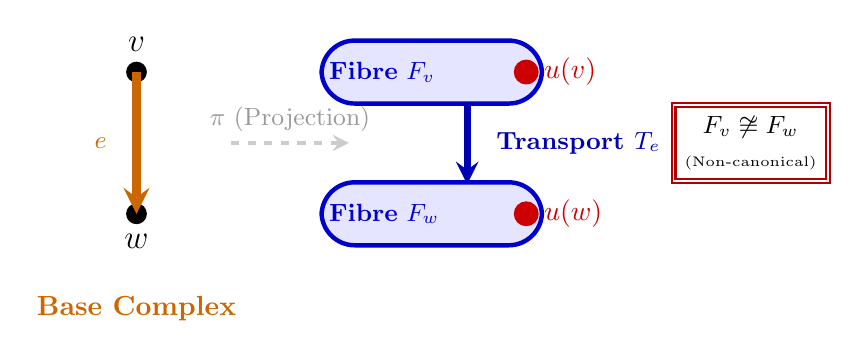
\begin{tikzpicture}[scale=1.5, every node/.style={font=\small}, >=stealth]

% --- LEFT SECTION: GEOMETRIC BASE (The Mesh) ---
\begin{scope}[shift={(0, 0)}]
    \coordinate (v) at (0, 1.2);
    \coordinate (w) at (0, 0);

    % Vertices
    \fill[black] (v) circle (2.5pt) node[above=4pt] {\large $v$};
    \fill[black] (w) circle (2.5pt) node[below=4pt] {\large $w$};

    % Edge
    \draw[line width=3pt, orange!80!black, ->] (v) -- (w)
        node[midway, left=6pt, font=\small\bfseries] {$e$};

    \node[orange!80!black, font=\bfseries\scshape] at (0, -0.8) {Base Complex};
\end{scope}

% --- TRANSITION: PROJECTION ---
\draw[->, dashed, ultra thick, gray!40] (0.8, 0.6) -- (1.8, 0.6)
    node[midway, above, gray!80] {$\pi$ (Projection)};

% --- RIGHT SECTION: ALGEBRAIC FIBRES (The Abstract Space) ---
\begin{scope}[shift={(2.5, 0)}]
    % Fibre over v
    \node[draw, ultra thick, rounded corners=12pt, fill=blue!10, 
          minimum width=2.8cm, minimum height=0.8cm, draw=blue!80!black] 
          (Fv) at (0, 1.2) {};
    \node[anchor=west, blue!80!black] at (Fv.west) {\small \textbf{Fibre} $F_v$};

    % Fibre over w
    \node[draw, ultra thick, rounded corners=12pt, fill=blue!10, 
          minimum width=2.8cm, minimum height=0.8cm, draw=blue!80!black] 
          (Fw) at (0, 0) {};
    \node[anchor=west, blue!80!black] at (Fw.west) {\small \textbf{Fibre} $F_w$};

    % Sections (Node States)
    \fill[red!80!black] (Fv.center) +(0.8,0) circle (3pt) 
        node[right=3pt, font=\bfseries] {$u(v)$};
    \fill[red!80!black] (Fw.center) +(0.8,0) circle (3pt) 
        node[right=3pt, font=\bfseries] {$u(w)$};

    % Connection / Transport Map
    \draw[->, line width=2.5pt, blue!70!black] (0.3, 0.95) -- (0.3, 0.25)
        node[midway, right=6pt, font=\small\bfseries] {Transport $T_e$};

    % Non-canonical marker
    \node[draw=red!70!black, fill=white, thick, double, inner sep=4pt, align=center] 
        at (2.7, 0.6)
        {\small $F_v \not\cong F_w$ \\[1pt] \tiny (Non-canonical)};
\end{scope}

\end{tikzpicture}

\end{frame}

% ---------------- Slide 17 — Transport along edges (reframe as groupoid representation) ----------------
\begin{frame}{Transport along edges: a groupoid viewpoint}
\begin{itemize}
\item The 1-skeleton paths form a \textbf{path groupoid} (objects = vertices, morphisms = paths).
\item A connection is an assignment of linear maps to generating morphisms (edges), extended by composition.
\item Curvature appears when the 2-cells impose relations that are not respected by the transport (holonomy defect).
\end{itemize}
% This slide makes the later curvature slide feel inevitable and “geometric”.

\begin{center}
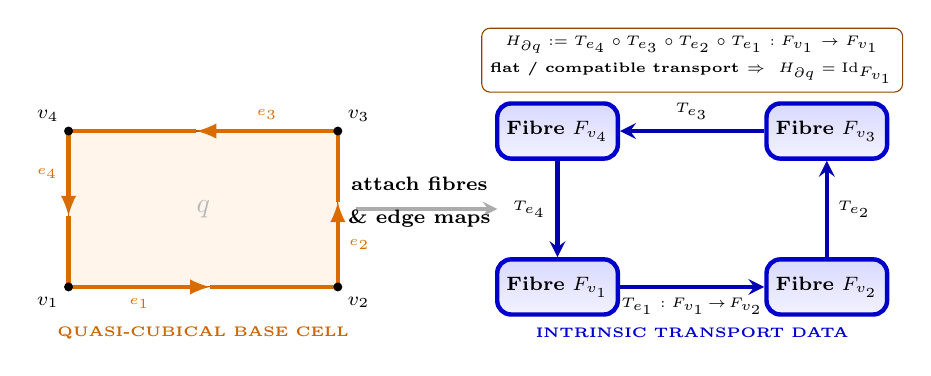
\begin{tikzpicture}[scale=0.9, every node/.style={font=\scriptsize}]

% ===================== LEFT: QUASI-CUBICAL BASE MESH =====================
\begin{scope}[shift={(0,0)}]
    % Face
    \fill[orange!10, opacity=0.8] (0,0)--(3.8,0)--(3.8,2.2)--(0,2.2)--cycle;
    \draw[orange!60!black, thin] (0,0)--(3.8,0)--(3.8,2.2)--(0,2.2)--cycle;

    % Oriented boundary edges
    \draw[->, >=latex, line width=1.5pt, orange!85!black] (0,0) -- (2.0,0)
        node[midway, below, font=\tiny] {$e_1$};
    \draw[line width=1.5pt, orange!85!black] (2.0,0) -- (3.8,0);

    \draw[->, >=latex, line width=1.5pt, orange!85!black] (3.8,0) -- (3.8,1.2)
        node[midway, right, font=\tiny] {$e_2$};
    \draw[line width=1.5pt, orange!85!black] (3.8,1.2) -- (3.8,2.2);

    \draw[->, >=latex, line width=1.5pt, orange!85!black] (3.8,2.2) -- (1.8,2.2)
        node[midway, above, font=\tiny] {$e_3$};
    \draw[line width=1.5pt, orange!85!black] (1.8,2.2) -- (0,2.2);

    \draw[->, >=latex, line width=1.5pt, orange!85!black] (0,2.2) -- (0,1.0)
        node[midway, left, font=\tiny] {$e_4$};
    \draw[line width=1.5pt, orange!85!black] (0,1.0) -- (0,0);

    % Vertices
    \fill[black] (0,0) circle (1.8pt) node[below left] {$v_1$};
    \fill[black] (3.8,0) circle (1.8pt) node[below right] {$v_2$};
    \fill[black] (3.8,2.2) circle (1.8pt) node[above right] {$v_3$};
    \fill[black] (0,2.2) circle (1.8pt) node[above left] {$v_4$};

    % Face label
    \node[gray!55, font=\itshape] at (1.9,1.1) {$q$};

    % Title
    \node[font=\tiny\bfseries, orange!80!black] at (1.9,-0.65) {QUASI-CUBICAL BASE CELL};
\end{scope}

% ===================== MIDDLE: CORRESPONDENCE =====================
\begin{scope}[shift={(5.25,1.1)}]
    \draw[->, >=stealth, line width=1.3pt, gray!65] (-1.2,0) -- (0.8,0);
    \node[above, font=\scriptsize\bfseries] at (-0.3, 0.12) {attach fibres};
    \node[below, font=\scriptsize\bfseries] at (-0.3, 0.12) {\& edge maps};
\end{scope}

% ===================== RIGHT: FIBRE / TRANSPORT DATA =====================
\begin{scope}[shift={(6.9, 0)}]
    % Fibre boxes
    \node[rounded corners=5pt, draw=blue!80!black, ultra thick,
          top color=blue!15, bottom color=blue!5,
          minimum width=1.45cm, minimum height=0.7cm] (F1) at (0,0) {\textbf{Fibre} $F_{v_1}$};

    \node[rounded corners=5pt, draw=blue!80!black, ultra thick,
          top color=blue!15, bottom color=blue!5,
          minimum width=1.45cm, minimum height=0.7cm] (F2) at (3.8,0) {\textbf{Fibre} $F_{v_2}$};

    \node[rounded corners=5pt, draw=blue!80!black, ultra thick,
          top color=blue!15, bottom color=blue!5,
          minimum width=1.45cm, minimum height=0.7cm] (F3) at (3.8,2.2) {\textbf{Fibre} $F_{v_3}$};

    \node[rounded corners=5pt, draw=blue!80!black, ultra thick,
          top color=blue!15, bottom color=blue!5,
          minimum width=1.45cm, minimum height=0.7cm] (F4) at (0,2.2) {\textbf{Fibre} $F_{v_4}$};

    % Transport maps along oriented edges
    \draw[->, >=stealth, line width=1.5pt, blue!70!black] (F1.east) -- (F2.west)
        node[midway, below, text=black, font=\tiny] {$T_{e_1}:F_{v_1}\!\to\!F_{v_2}$};

    \draw[->, >=stealth, line width=1.5pt, blue!70!black] (F2.north) -- (F3.south)
        node[midway, right, text=black, font=\tiny] {$T_{e_2}$};

    \draw[->, >=stealth, line width=1.5pt, blue!70!black] (F3.west) -- (F4.east)
        node[midway, above, text=black, font=\tiny] {$T_{e_3}$};

    \draw[->, >=stealth, line width=1.5pt, blue!70!black] (F4.south) -- (F1.north)
        node[midway, left, text=black, font=\tiny] {$T_{e_4}$};

    % Holonomy / compatibility box
    \node[fill=white, draw=orange!55!black, rounded corners=3pt,
          inner sep=3pt, align=center, font=\tiny\bfseries] at (1.9, 3.2)
    {$H_{\partial q}:=T_{e_4}\circ T_{e_3}\circ T_{e_2}\circ T_{e_1}:F_{v_1}\to F_{v_1}$\\[2pt]
     flat / compatible transport $\Rightarrow\ H_{\partial q}=\mathrm{Id}_{F_{v_1}}$};

    % Title
    \node[font=\tiny\bfseries, blue!80!black] at (1.9,-0.65) {INTRINSIC TRANSPORT DATA};
\end{scope}

\end{tikzpicture}
\end{center}

\end{frame}

% ============================================================
% PART V — Obstructions: curvature, torsion-like defects, and algebra
% ============================================================
\section{Obstructions and algebraic structure}

% ---------------- Slide 18 — Curvature as holonomy defect (move curvature earlier; separate from bracket) ----------------
\begin{frame}{Curvature as holonomy defect (primary notion)}
\begin{itemize}
\item A 2-cell determines a closed boundary walk in the 1-skeleton.
\item Parallel transport around that loop yields an endomorphism of a fibre (holonomy).
\item \textbf{Curvature:} deviation of holonomy from identity (or from a reference transport).
\end{itemize}
% Keep ONE loop picture; remove the large formula badges.

\begin{center}
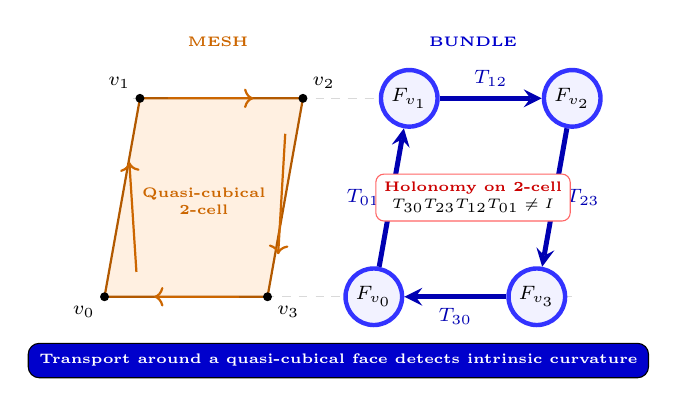
\begin{tikzpicture}[scale=0.9, every node/.style={font=\scriptsize}]

% --- PROJECTION LINES (Connecting the layers) ---
\draw[dashed, gray!30, thin] (0,0) -- (3.4,0);
\draw[dashed, gray!30, thin] (0,2.8) -- (3.4,2.8);
\draw[dashed, gray!30, thin] (2.8,0) -- (6.2,0);
\draw[dashed, gray!30, thin] (2.8,2.8) -- (6.2,2.8);

% --- LEFT LAYER: THE GEOMETRY (Quasi-cubical face) ---
\begin{scope}[shift={(-0.4,0)}]
    % Face shading
    \fill[orange!15, opacity=0.8] (0,0) -- (0.5,2.8) -- (2.8,2.8) -- (2.3,0) -- cycle;
    \draw[orange!70!black, thick] (0,0) -- (0.5,2.8) -- (2.8,2.8) -- (2.3,0) -- cycle;

    % Vertices
    \fill[black] (0,0) circle (1.8pt) node[below left] {$v_0$};
    \fill[black] (0.5,2.8) circle (1.8pt) node[above left] {$v_1$};
    \fill[black] (2.8,2.8) circle (1.8pt) node[above right] {$v_2$};
    \fill[black] (2.3,0) circle (1.8pt) node[below right] {$v_3$};

    % Boundary orientation
    \draw[->, thick, orange!80!black] (0.45,0.35) -- (0.35,1.9);
    \draw[->, thick, orange!80!black] (0.9,2.8) -- (2.1,2.8);
    \draw[->, thick, orange!80!black] (2.55,2.3) -- (2.45,0.6);
    \draw[->, thick, orange!80!black] (1.9,0) -- (0.7,0);

    \node[orange!80!black, font=\tiny\bfseries, align=center] at (1.4,1.35) {Quasi-cubical\\2-cell};
\end{scope}

% --- RIGHT LAYER: THE TRANSPORT (Fibre/Algebraic) ---
\begin{scope}[shift={(3.4,0)}]
    % Nodes/Fibres
    \node[circle, draw=blue!80, ultra thick, fill=blue!5, inner sep=2pt] (F0) at (0,0) {$F_{v_0}$};
    \node[circle, draw=blue!80, ultra thick, fill=blue!5, inner sep=2pt] (F1) at (0.5,2.8) {$F_{v_1}$};
    \node[circle, draw=blue!80, ultra thick, fill=blue!5, inner sep=2pt] (F2) at (2.8,2.8) {$F_{v_2}$};
    \node[circle, draw=blue!80, ultra thick, fill=blue!5, inner sep=2pt] (F3) at (2.3,0) {$F_{v_3}$};

    % Transport maps around boundary
    \draw[->, >=stealth, line width=1.8pt, blue!70!black] (F0) -- (F1) node[midway, left] {$T_{01}$};
    \draw[->, >=stealth, line width=1.8pt, blue!70!black] (F1) -- (F2) node[midway, above] {$T_{12}$};
    \draw[->, >=stealth, line width=1.8pt, blue!70!black] (F2) -- (F3) node[midway, right] {$T_{23}$};
    \draw[->, >=stealth, line width=1.8pt, blue!70!black] (F3) -- (F0) node[midway, below] {$T_{30}$};

    % Holonomy / curvature label
    \node[
        fill=white,
        draw=red!60,
        rounded corners=3pt,
        inner sep=3pt,
        font=\tiny\bfseries,
        align=center
    ] at (1.4,1.4)
    {\color{red!80!black} Holonomy on 2-cell\\$T_{30}T_{23}T_{12}T_{01}\neq I$};
\end{scope}

% --- CATCHY ANALYSIS BOX ---
\node[
    draw,
    rounded corners=4pt,
    fill=blue!80!black,
    text=white,
    inner sep=4pt,
    align=center,
    font=\tiny\bfseries
] at (2.9,-0.9)
{Transport around a quasi-cubical face detects intrinsic curvature};

% --- TOP ANNOTATIONS ---
\node[orange!80!black, font=\tiny\bfseries] at (1.2,3.6) {MESH};
\node[blue!80!black, font=\tiny\bfseries] at (4.8,3.6) {BUNDLE};

\end{tikzpicture}
\end{center}

\end{frame}

% ---------------- Slide 19 — Torsion-like obstruction (rename unless you add soldering) ----------------
\begin{frame}{A torsion-like obstruction (compatibility defect)}
\begin{itemize}
\item Measures failure of a chosen “direct” transport to agree with composed transport along a 2-step path.
\item Interpretable as \textbf{compatibility defect} tied to incidence + transport choices.
\item If you want to call it torsion: specify the additional structure (frame/soldering) it refers to.
\end{itemize}
% Keep the triangle picture if you like; remove strong claims equating it to torsion in Cartan sense.

\begin{center}
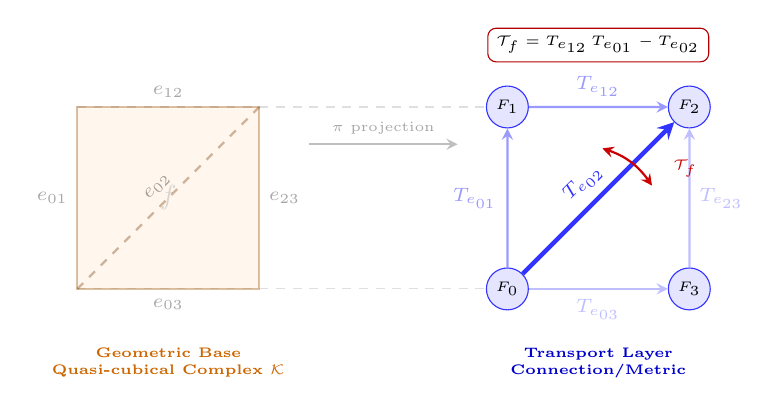
\begin{tikzpicture}[scale=1.05, every node/.style={font=\scriptsize}, >=stealth]

% =========================================================
% Quasi-cubical example: square face with one diagonal path
% =========================================================

% --- 1. COORDINATE DEFINITION (Horizontal Layout) ---
% Left layer: Geometric Base (quasi-cubical face)
\coordinate (v0_left) at (0,0);
\coordinate (v1_left) at (0,2.2);
\coordinate (v2_left) at (2.2,2.2);
\coordinate (v3_left) at (2.2,0);

% Right layer: Transport Layer
\coordinate (v0_right) at (5.2,0);
\coordinate (v1_right) at (5.2,2.2);
\coordinate (v2_right) at (7.4,2.2);
\coordinate (v3_right) at (7.4,0);

% --- 2. HORIZONTAL PROJECTIONS (The "Coupling") ---
\draw[dashed, gray!25] (v0_left) -- (v0_right);
\draw[dashed, gray!25] (v1_left) -- (v1_right);
\draw[dashed, gray!25] (v2_left) -- (v2_right);
\draw[dashed, gray!25] (v3_left) -- (v3_right);

% --- 3. LEFT LAYER: GEOMETRIC BASE (Faded Background) ---
\begin{scope}[opacity=0.35]
    \fill[orange!20] (v0_left)--(v1_left)--(v2_left)--(v3_left)--cycle;
    \draw[orange!60!black, thick] (v0_left)--(v1_left)--(v2_left)--(v3_left)--cycle;
    
    % Optional diagonal for comparison path
    \draw[orange!45!black, thick, dashed] (v0_left)--(v2_left);

    % Edge labels
    \path (v0_left) -- (v1_left) node[midway, left] {$e_{01}$};
    \path (v1_left) -- (v2_left) node[midway, above] {$e_{12}$};
    \path (v2_left) -- (v3_left) node[midway, right] {$e_{23}$};
    \path (v0_left) -- (v3_left) node[midway, below] {$e_{03}$};
    \path (v0_left) -- (v2_left) node[midway, sloped, above] {$e_{02}$};

    \node[gray!80, font=\bfseries] at (1.1,1.1) {$f$};
\end{scope}

% Left layer label
\node[anchor=north, orange!80!black, align=center, font=\tiny\bfseries] at (1.1,-0.6) 
    {Geometric Base\\Quasi-cubical Complex $\mathcal{K}$};

% --- 4. RIGHT LAYER: TRANSPORT LAYER (Highlighted Foreground) ---
\begin{scope}
    % Fiber Nodes
    \node[circle, draw=blue!80, fill=blue!10, inner sep=2pt, font=\tiny\bfseries] (F0) at (v0_right) {$F_0$};
    \node[circle, draw=blue!80, fill=blue!10, inner sep=2pt, font=\tiny\bfseries] (F1) at (v1_right) {$F_1$};
    \node[circle, draw=blue!80, fill=blue!10, inner sep=2pt, font=\tiny\bfseries] (F2) at (v2_right) {$F_2$};
    \node[circle, draw=blue!80, fill=blue!10, inner sep=2pt, font=\tiny\bfseries] (F3) at (v3_right) {$F_3$};

    % Reference Path (diagonal transport)
    \draw[->, ultra thick, blue!80] (F0) -- (F2)
        node[midway, sloped, above] {$T_{e_{02}}$};

    % Comparison Path (two-step transport around the square)
    \draw[->, thick, blue!40] (F0) -- (F1)
        node[midway, left] {$T_{e_{01}}$};
    \draw[->, thick, blue!40] (F1) -- (F2)
        node[midway, above] {$T_{e_{12}}$};

    % Alternative longer path (optional visual cue)
    \draw[->, thick, blue!25] (F0) -- (F3)
        node[midway, below] {$T_{e_{03}}$};
    \draw[->, thick, blue!25] (F3) -- (F2)
        node[midway, right] {$T_{e_{23}}$};

    % Torsion/defect indicator
    \draw[<->, red!80!black, thick, bend right=20] (6.95,1.25) to (6.35,1.7);
    \node[red!80!black, font=\tiny\bfseries] at (7.35,1.45) {$\mathcal{T}_f$};

    % Equation badge
    \node[draw=red!70!black, fill=white, rounded corners=3pt,
          inner sep=3pt, font=\tiny\bfseries, align=center] at (6.3,2.95)
        {$\mathcal{T}_f = T_{e_{12}}\,T_{e_{01}} - T_{e_{02}}$};
\end{scope}

% Right layer label
\node[anchor=north, blue!80!black, align=center, font=\tiny\bfseries] at (6.3,-0.6) 
    {Transport Layer\\Connection/Metric};

% --- 5. CONNECTION ARROWS ---
\draw[->, thick, gray!50] (2.8,1.75) -- (4.6,1.75)
    node[midway, above, gray!70, font=\tiny] {$\pi$ projection};

\end{tikzpicture}
\end{center}
\end{frame}

% ---------------- Slide 20 — Antisymmetric bracket (keep, but soften claims) ----------------
\begin{frame}{An antisymmetric bracket on sections (current work)
\href{https://kipiberbatov.github.io/cmc/main.pdf}{\beamergotobutton{Berbatov 2026}}
}
\begin{itemize}
\item Define an antisymmetric bilinear operation on vector-valued 0-forms using incidence + transport.
\item The Jacobiator provides an \textbf{algebraic obstruction} (generally nonzero).
\item This obstruction is a candidate invariant; its precise relation to curvature/torsion is an open question.
\end{itemize}
% Remove the full bilinear/Jacobi equations; keep only the conceptual properties.
% Do NOT visually label “curvature = J != 0” on this slide.


\centering
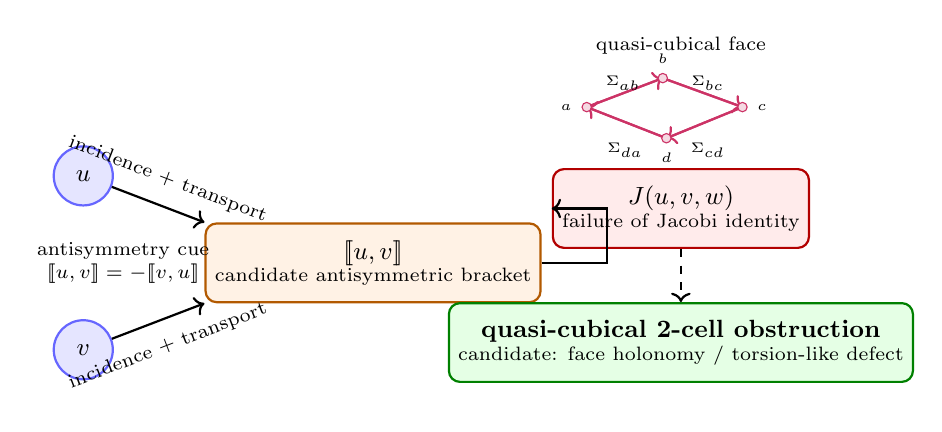
\begin{tikzpicture}[
    scale=0.92,
    every node/.style={font=\small},
    section/.style={circle, draw=blue!60, fill=blue!10, thick, minimum size=7.5mm},
    opbox/.style={rounded corners, draw=orange!70!black, fill=orange!10, thick, minimum width=3.0cm, minimum height=1.0cm, align=center},
    obsbox/.style={rounded corners, draw=red!70!black, fill=red!8, thick, minimum width=3.0cm, minimum height=1.0cm, align=center},
    candbox/.style={rounded corners, draw=green!50!black, fill=green!10, thick, minimum width=4.2cm, minimum height=1.0cm, align=center},
    arr/.style={->, thick},
    dashedarr/.style={->, thick, dashed}
]

% Left: sections
\node[section] (u) at (0,1.2) {$u$};
\node[section] (v) at (0,-1.2) {$v$};

% Middle: bracket
\node[opbox] (bracket) at (4.0,0) {$[\![u,v]\!]$\\[-1mm]\scriptsize candidate antisymmetric bracket};

\draw[arr] (u) -- node[above, sloped, yshift=1mm] {\scriptsize incidence $+$ transport} (bracket.north west);
\draw[arr] (v) -- node[below, sloped, yshift=-1mm] {\scriptsize incidence $+$ transport} (bracket.south west);

\node[align=center] at (0.55, 0) {\scriptsize antisymmetry cue\\[-1mm]\scriptsize $[\![u,v]\!] = -[\![v,u]\!]$};

% Right: Jacobiator and obstruction
\node[obsbox] (jac) at (8.25, 0.75) {$J(u,v,w)$\\[-1mm]\scriptsize failure of Jacobi identity};
\node[candbox] (obs) at (8.25, -1.10) {\textbf{quasi-cubical 2-cell obstruction}\\[-1mm]\scriptsize candidate: face holonomy / torsion-like defect};

\draw[arr] (bracket.east) -- ++(0.9,0) |- (jac.west);
\draw[dashedarr] (jac.south) -- (obs.north);

% Top-right: quasi-cubical face sketch
\node[font=\scriptsize] at (8.25,3.0) {quasi-cubical face};

\coordinate (a) at (6.95,2.15);
\coordinate (b) at (8.00,2.55);
\coordinate (c) at (9.10,2.15);
\coordinate (d) at (8.05,1.72);

\draw[thick, purple!80] (a) -- (b) -- (c) -- (d) -- cycle;
\draw[->, thick, purple!80] (a) -- (b);
\draw[->, thick, purple!80] (b) -- (c);
\draw[->, thick, purple!80] (c) -- (d);
\draw[->, thick, purple!80] (d) -- (a);

\node[circle, fill=purple!15, draw=purple!80, inner sep=1.2pt, label=left:{\tiny $a$}] at (a) {};
\node[circle, fill=purple!15, draw=purple!80, inner sep=1.2pt, label=above:{\tiny $b$}] at (b) {};
\node[circle, fill=purple!15, draw=purple!80, inner sep=1.2pt, label=right:{\tiny $c$}] at (c) {};
\node[circle, fill=purple!15, draw=purple!80, inner sep=1.2pt, label=below:{\tiny $d$}] at (d) {};

\node[font=\tiny] at (7.45,2.48) {$\Sigma_{ab}$};
\node[font=\tiny] at (8.62,2.48) {$\Sigma_{bc}$};
\node[font=\tiny] at (8.62,1.55) {$\Sigma_{cd}$};
\node[font=\tiny] at (7.48,1.55) {$\Sigma_{da}$};

\end{tikzpicture}
\end{frame}

% ---------------- Slide 21 — Invariants and gauge (NEW; geometers will ask this) ----------------
\begin{frame}{Invariants and gauge (what should be classified?)}
\begin{itemize}
\item Gauge change: re-choose bases in each $F_v$ (vertex-wise change of frames).
\item Holonomy classes around 2-cells: conjugacy-type invariants under gauge.
\item Cohomological data (scalar sector) vs holonomy/obstruction data (vector sector).
\end{itemize}
% This slide turns Q&A into productive math discussion rather than “is this useful?”.

\centering
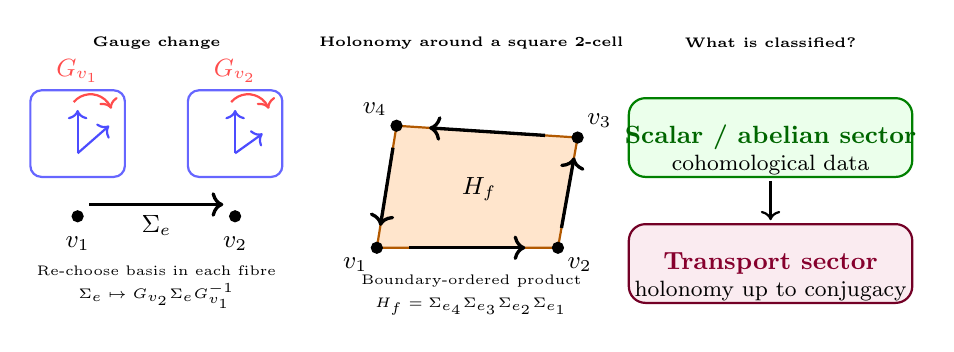
\begin{tikzpicture}[scale=1.0, every node/.style={font=\small}]
    % ---------------- Left: gauge change ----------------
    \begin{scope}[shift={(-4.8, 0)}]
        \node[font=\bfseries] at (0,2.2) {\tiny Gauge change};

        % vertices
        \filldraw[black] (-1,0) circle (2pt) node[below=4pt] {$v_1$};
        \filldraw[black] (1,0) circle (2pt) node[below=4pt] {$v_2$};

        % fibres
        \draw[rounded corners=4pt, thick, blue!60] (-1.6,0.5) rectangle (-0.4,1.6);
        \draw[rounded corners=4pt, thick, blue!60] (0.4,0.5) rectangle (1.6,1.6);

        % local basis arrows
        \draw[->, thick, blue!70] (-1,0.8) -- (-1,1.35);
        \draw[->, thick, blue!70] (-1,0.8) -- (-0.6,1.15);
        \draw[->, thick, blue!70] (1,0.8) -- (1,1.35);
        \draw[->, thick, blue!70] (1,0.8) -- (1.35,1.05);

        % edge transport
        \draw[->, very thick] (-0.85,0.15) -- (0.85,0.15) node[midway, below] {$\Sigma_e$};

        % gauge rotation marks
        \draw[->, red!70, thick] (-1.05,1.45) arc[start angle=140,end angle=20,radius=0.28];
        \draw[->, red!70, thick] (0.95,1.45) arc[start angle=140,end angle=20,radius=0.28];

        \node[red!70] at (-1,1.85) {$G_{v_1}$};
        \node[red!70] at (1,1.85) {$G_{v_2}$};

        \node[align=center] at (0,-0.9) {\tiny Re-choose basis in each fibre\\[-1mm]
        \tiny $\Sigma_e \mapsto G_{v_2}\Sigma_e G_{v_1}^{-1}$};
    \end{scope}

    % ---------------- Center: holonomy on a quasi-cubical 2-cell ----------------
    \begin{scope}[shift={(-0.8, 0)}]
        \node[font=\bfseries] at (0,2.2) {\tiny Holonomy around a square 2-cell};

        % quasi-cubical face
        \coordinate (a) at (-1.2,-0.4);
        \coordinate (b) at (1.1,-0.4);
        \coordinate (c) at (1.35,1.0);
        \coordinate (d) at (-0.95,1.15);

        \filldraw[orange!20, draw=orange!70!black, thick] (a)--(b)--(c)--(d)--cycle;

        \filldraw[black] (a) circle (2pt) node[below left] {$v_1$};
        \filldraw[black] (b) circle (2pt) node[below right] {$v_2$};
        \filldraw[black] (c) circle (2pt) node[above right] {$v_3$};
        \filldraw[black] (d) circle (2pt) node[above left] {$v_4$};

        % oriented transport arrows around boundary
        \draw[->, very thick] ($(a)!0.18!(b)$) -- ($(a)!0.82!(b)$);
        \draw[->, very thick] ($(b)!0.18!(c)$) -- ($(b)!0.82!(c)$);
        \draw[->, very thick] ($(c)!0.18!(d)$) -- ($(c)!0.82!(d)$);
        \draw[->, very thick] ($(d)!0.18!(a)$) -- ($(d)!0.82!(a)$);

        \node at (0.1,0.35) {$H_f$};
        \node[align=center] at (0,-1.0) {\tiny Boundary-ordered product\\[-1mm]
        \tiny $H_f=\Sigma_{e_4}\Sigma_{e_3}\Sigma_{e_2}\Sigma_{e_1}$};
    \end{scope}

    % ---------------- Right: classification split ----------------
    \begin{scope}[shift={(3.0, 0)}]
        \node[font=\bfseries] at (0,2.2) {\tiny What is classified?};

        % scalar / abelian box
        \draw[rounded corners=6pt, thick, green!50!black, fill=green!8] (-1.8,0.5) rectangle (1.8,1.5);
        \node[green!40!black] at (0,1.0) {\textbf{Scalar / abelian sector}};
        \node at (0,0.65) {\footnotesize cohomological data};

        % transport / gauge box
        \draw[rounded corners=6pt, thick, purple!60!black, fill=purple!8] (-1.8,-1.1) rectangle (1.8,-0.1);
        \node[purple!70!black] at (0,-0.6) {\textbf{Transport sector}};
        \node at (0,-0.95) {\footnotesize holonomy up to conjugacy};

        % separator arrow
        \draw[->, thick] (0,0.45) -- (0,-0.05);
    \end{scope}
\end{tikzpicture}

\vspace{0.5em}
{\footnotesize For scalar/abelian transport one expects \textcolor{green!40!black}{cohomological invariants}, whereas for general bundle-valued transport the intrinsic gauge-invariant data is \textcolor{purple!70!black}{holonomy up to conjugacy}.}

\end{frame}

% ============================================================
% PART VI — Brief mechanics motivation + open problems
% ============================================================
\section{Outlook}

% ---------------- Slide 22 — Brief mechanics motivation (one slide only; keep modest) ----------------
\begin{frame}{Why mechanics cares (brief motivation)}
\begin{itemize}
\item Forces/defects concentrate on lower-dimensional features (interfaces, junctions): naturally “cell-supported”.
\item Transport inconsistencies (holonomy/compatibility defects) suggest a geometric language for internal structure.
\item This is motivation only; the mathematical development is the focus of this seminar.
\end{itemize}
% Remove the multi-panel infographic; it reads like a grant slide, not a math seminar.

\vspace{-0.5cm}
\begin{center}
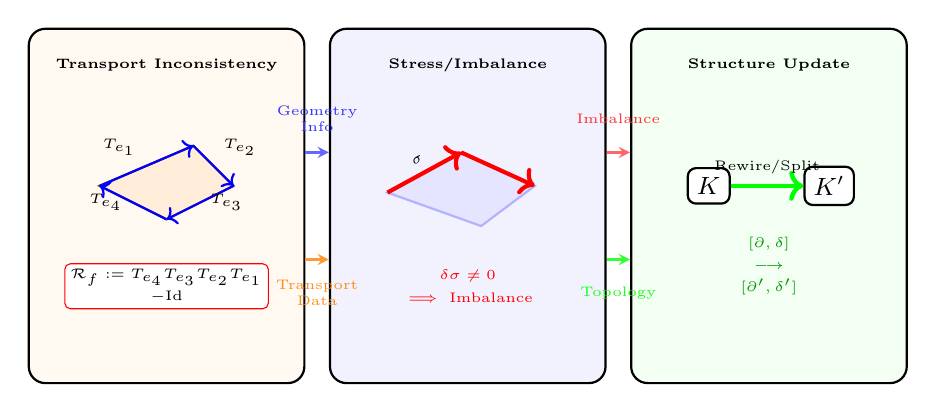
\begin{tikzpicture}[scale=0.85, every node/.style={font=\scriptsize}]
% ---------------- Background Panels (Horizontal Layout) ----------------
\node[draw, rounded corners=6pt, thick, fill=orange!5, minimum width=3.5cm, minimum height=4.5cm] (P1) at (0, 0) {};
\node[draw, rounded corners=6pt, thick, fill=blue!5, minimum width=3.5cm, minimum height=4.5cm] (P2) at (4.5, 0) {};
\node[draw, rounded corners=6pt, thick, fill=green!5, minimum width=3.5cm, minimum height=4.5cm] (P3) at (9, 0) {};

% ---------------- Flow Connectors (Horizontal) ----------------
\draw[->, >=stealth, thick, draw=blue!60]
    ([yshift=0.8cm]P1.east) -- ([yshift=0.8cm]P2.west);
\draw[->, >=stealth, thick, draw=orange!80]
    ([yshift=-0.8cm]P1.east) -- ([yshift=-0.8cm]P2.west);

\node[font=\tiny, text=blue!80, align=center] at (2.25, 1.3) {Geometry\\Info};
\node[font=\tiny, text=orange!90, align=center] at (2.25, -1.3) {Transport\\Data};

\draw[->, >=stealth, thick, draw=red!60]
    ([yshift=0.8cm]P2.east) -- ([yshift=0.8cm]P3.west);
\draw[->, >=stealth, thick, draw=green!80]
    ([yshift=-0.8cm]P2.east) -- ([yshift=-0.8cm]P3.west);

\node[font=\tiny, text=red!80, align=center] at (6.75, 1.3) {Imbalance};
\node[font=\tiny, text=green!90, align=center] at (6.75, -1.3) {Topology};

% =========================================================
% (1) Transport Inconsistency
% =========================================================
\begin{scope}[shift={(0, 0)}]
    \node[anchor=north, font=\bfseries, align=center] at (0, 2.35) {\tiny Transport Inconsistency};
    \coordinate (A) at (-1.0, 0.3); \coordinate (B) at (0.4, 0.9);
    \coordinate (C) at (1.0, 0.3);  \coordinate (D) at (0, -0.2);

    \fill[orange!15] (A)--(B)--(C)--(D)--cycle;
    \draw[orange!50!black, thick] (A)--(B)--(C)--(D)--cycle;

    \draw[->, thick, draw=blue] (A) -- (B) node[midway, above left] {\tiny $T_{e_1}$};
    \draw[->, thick, draw=blue] (B) -- (C) node[midway, above right] {\tiny $T_{e_2}$};
    \draw[->, thick, draw=blue] (C) -- (D) node[midway, right] {\tiny $T_{e_3}$};
    \draw[->, thick, draw=blue] (D) -- (A) node[midway, left] {\tiny $T_{e_4}$};

    \node[fill=white, inner sep=2pt, draw=red, rounded corners=2pt, align=center] at (0, -1.2)
        {\tiny $\mathcal{R}_f := T_{e_4}T_{e_3}T_{e_2}T_{e_1}$\\\tiny $-\mathrm{Id}$};
\end{scope}

% =========================================================
% (2) Stress Indicator (Topological)
% =========================================================
\begin{scope}[shift={(4.5, 0)}]
    \node[anchor=north, font=\bfseries, align=center] at (0, 2.35) {\tiny Stress/Imbalance};
    \coordinate (v0) at (-1.2, 0.2); \coordinate (v1) at (-0.1, 0.8);
    \coordinate (v2) at (1.0, 0.3);  \coordinate (v3) at (0.2, -0.3);

    \fill[blue!10] (v0)--(v1)--(v2)--(v3)--cycle;
    \draw[blue!30, thick] (v0)--(v1)--(v2)--(v3)--cycle;

    \draw[line width=1.5pt, draw=red, ->] (v0)--(v1) node[midway, sloped, above] {\tiny $\sigma$};
    \draw[line width=1.5pt, draw=red, ->] (v1)--(v2);

    \node[anchor=center, text=red, align=center] at (0, -1.2) {\tiny $\delta\sigma \neq 0$\\\tiny $\implies \text{Imbalance}$};
\end{scope}

% =========================================================
% (3) Structure Update (Evolution)
% =========================================================
\begin{scope}[shift={(9, 0)}]
    \node[anchor=north, font=\bfseries, align=center] at (0, 2.35) {\tiny Structure Update};

    \node[draw, rounded corners=3pt, fill=white, thick] (K)  at (-0.9, 0.3) {\small $K$};
    \node[draw, rounded corners=3pt, fill=white, thick] (Kp) at (0.9, 0.3)  {\small $K'$};

    \draw[->, ultra thick, draw=green] (K) -- (Kp)
        node[midway, above, font=\tiny, text=black] {Rewire/Split};

    \node[text=green!60!black, align=center] at (0, -0.9)
        {\tiny $[\partial, \delta]$\\\tiny $\longrightarrow$\\\tiny $[\partial', \delta']$};
\end{scope}

\end{tikzpicture}
\end{center}

\end{frame}

% ---------------- Slide 23 — Open mathematical questions (tighten) ----------------
\begin{frame}{Open mathematical questions}
\begin{itemize}
\item What is the right class of admissible edge transports when fibre ranks vary?
\item What are the right curvature/holonomy invariants under gauge and refinement?
\item How should torsion be defined (what additional structure is required)?
\item How do these structures behave under the evolution of $K$ (rewiring, splitting, refinement)?
\end{itemize}
\end{frame}

% ---------------- Slide 24 — Closing (remove slogans; end with a question) ----------------
\begin{frame}{Closing}
\begin{itemize}
\item Cochains provide an intrinsic calculus on a finite complex (topology first, metric optional).
\item Vector-valued quantities force us to confront transport/connection as \emph{extra structure}.
\item \textbf{Closing question:} which obstructions (holonomy, Jacobiator, torsion-like defects) are the right “geometry” of a combinatorial system?
\end{itemize}

\begin{center}

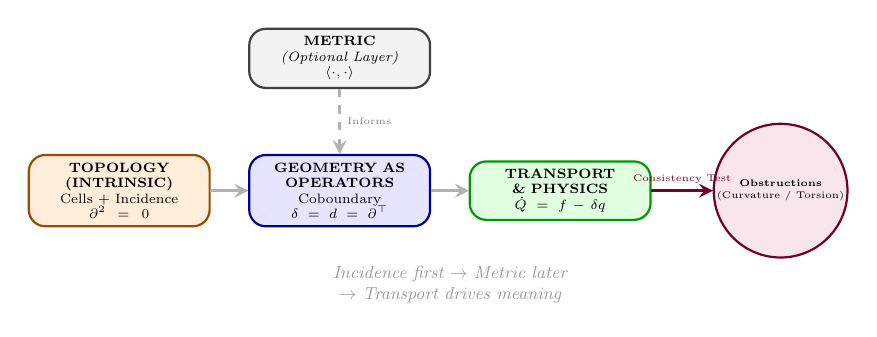
\begin{tikzpicture}[
    scale=0.7, transform shape,
    box/.style={draw, thick, rounded corners=6pt, inner sep=4pt, text width=3cm, minimum height=0.9cm, align=center, font=\scriptsize},
    arr/.style={->, >=stealth, line width=1.2pt, gray!60}
]

% --- HORIZONTAL ARCHITECTURE ---

% 1. Topology
\node[box, fill=orange!15, draw=orange!60!black] (topo) at (-6, 0)
{\textbf{TOPOLOGY (INTRINSIC)}\\
Cells + Incidence\\
$\partial^2 = 0$};

% 2. Geometry
\node[box, fill=blue!10, draw=blue!60!black] (ops) at (-2, 0)
{\textbf{GEOMETRY AS OPERATORS}\\
Coboundary $\delta = d = \partial^\top$};

% 3. Transport
\node[box, fill=green!12, draw=green!60!black] (trans) at (2, 0)
{\textbf{TRANSPORT \& PHYSICS}\\
$\dot{Q} = f - \delta q$};

% 4. Metric (optional layer above)
\node[box, fill=gray!10, draw=gray!50!black] (met) at (-2, 2.4)
{\textbf{METRIC}\\
\textit{(Optional Layer)}\\
$\langle \cdot, \cdot \rangle$};

% 5. Obstructions
\node[draw=purple!60!black, thick, circle, fill=purple!10, inner sep=1pt, font=\tiny, align=center] (obs) at (6, 0)
{\textbf{Obstructions}\\(Curvature / Torsion)};

% --- CONNECTIONS (Horizontal Flow) ---

\draw[arr] (topo) -- (ops);
\draw[arr] (ops) -- (trans);
\draw[arr, purple!60!black] (trans) -- (obs) node[midway, above, font=\tiny] {Consistency Test};

\draw[arr, dashed] (met) -- (ops) node[midway, right, font=\tiny, text=gray] {Informs};

% --- CAPTION ---
\node[font=\small\itshape, text width=7cm, text=gray!80, align=center] at (0, -1.7)
{Incidence first $\rightarrow$ Metric later $\rightarrow$ Transport drives meaning};

\end{tikzpicture}

\end{center}
\end{frame}

% ---------------- Slide 25 — Thank you (plain) ----------------
% \begin{frame}[plain]
% \centering
% \vfill
% {\Large \bfseries Thank you.}\\[0.25cm]
% {\small Questions and comments welcome.}
% \vfill
% \end{frame}

\begin{frame}[allowframebreaks]{References}
\footnotesize

\begin{thebibliography}{9}

\bibitem{Forman2002}
R. Forman (2002).  
\newblock \emph{Combinatorial Novikov--Morse Theory}.  
\newblock \textit{International Journal of Mathematics}, 13(4), 333--368.  
\newblock \href{https://www.worldscientific.com/doi/abs/10.1142/S0129167X02001265}{DOI link}

\vspace{0.2cm}

\bibitem{Berbatov2022}
K. Berbatov, P. D. Boom, A. L. Hazel, \& A. P. Jivkov (2022).  
\newblock \emph{Diffusion in Multi-dimensional Solids Using Forman’s Combinatorial Differential Forms}.  
\newblock \textit{Applied Mathematical Modelling}, 110, 172--192.  
\newblock \href{https://www.sciencedirect.com/science/article/pii/S0307904X22002657\#bib0023}{ScienceDirect}

\vspace{0.2cm}

\bibitem{BerbatovJivkov2025}
K. Berbatov \& A. P. Jivkov (2025).  
\newblock \emph{Variational Formulations of Transport Phenomena on Combinatorial Meshes}.  
\newblock arXiv preprint arXiv:2505.09443.  
\newblock \href{https://arxiv.org/abs/2505.09443}{arXiv}

\vspace{0.2cm}

\bibitem{Liu2025}
C. Liu, K. Berbatov, M. Sedighi, \& A. P. Jivkov (2025).  
\newblock \emph{Combinatorial Differential Forms for Multi-dimensional Fluid Flow in Porous Media:  
A Unified Framework for Volumetric Pores, Fractures, and Channels}.  
\newblock \textit{Advances in Water Resources}, Article 105095.  
\newblock \href{https://www.sciencedirect.com/science/article/pii/S030917082500209X}{ScienceDirect}

\vspace{0.2cm}

\bibitem{Liu2026}
C. Liu, A. Jivkov, K. Berbatov, M. Sedighi, J. Liu, \& H. Ni (2026).  
\newblock \emph{Microstructure-driven Prediction of Permeability and Thermal Conductivity in Porous Solids via a Discrete Multi-physics Framework}.  
\newblock \textit{International Journal of Rock Mechanics and Mining Sciences}, 199, 106432.  
\newblock \href{https://www.sciencedirect.com/science/article/pii/S1365160926000365}{ScienceDirect}

\vspace{0.2cm}

\bibitem{BerbatovCMC}
K. Berbatov.  
\newblock \emph{Combinatorial Mesh Calculus (CMC) Notes}.  
\newblock \href{https://kipiberbatov.github.io/cmc/main.pdf}{Online manuscript}

\end{thebibliography}

\end{frame}


\end{document}
